
\section{Positivity}\label{section: positivity}

In this section we prove \Cref{Teo D} from the introduction, and therefore verify \Cref{Conj A}.
More concretely, we prove that for any $\alpha_{i,j}\in \Phi^{\geq 2}$ and any $\lambda \in X^+$, the element $\bfM_{\lambda }^{\succ \alpha_{i,j}}$ can be written as a positive linear combination of elements of the form $\bfM_{\mu}^{\succeq \alpha_{i-k,j-k}}$ for $k\geq 0$, which is the content of \Cref{Teo D}.
From this, \Cref{Conj A} follows easily.

Let us briefly explain our strategy.
Our starting point is the Second Inverse Decomposition in \Cref{prop: second version refinado}.
We begin by isolating the term $\bfM_{\lambda}^{\succ \alpha_{i,j}}$ in \eqref{eq: SID ecuacion combi}.
We then have three cases to consider:
\begin{itemize}
\item The term $\bfM_{\mathbf{P}_{j,h}(\lambda)}^{\succ \alpha_{i,j}}$.

Since $\mathbf{P}_{j,h}(\lambda)< \lambda$ in the dominance order, we may assume by induction that \Cref{Teo D} holds for this weight.

\item The terms $X_m$ (defined in \eqref{eq: defi X in SID}). 

We refer to these terms as good pairs. 
We study these pairs in \Cref{section: good pairs}.
In particular, in \Cref{prop: caso bueno} we provide a positive combinatorial expansion of a term $X_m$ in terms of $\bfM_{\mu}^{\succeq \alpha_{i-m,j-m}}$-elements. 

\item The difference
\[
\bfM_{\mathbf{v}_{j,h}(\lambda)}^{\succ \alpha_{i,j}}
      - q^{e_2}\,  \bfM_{\mathbf{P}_{i,h}\mathbf{v}_{j,h}(\lambda)}^{\succ \alpha_{i,j}}.
\]

We observe that both weights involved in this difference are dominant. Therefore, we can apply \Cref{prop: second version refinado} again to these weights, and using an inductive argument, we conclude that this difference can also be written positively in terms of $\bfM$-elements.      
\end{itemize}




 


\subsection{Good Pairs} \label{section: good pairs}
In this section we obtain a positive combinatorial formula for the terms $X_m$ occurring in   \Cref{prop: second version refinado}. 
Our first step is the following technical lemma that will serve as the main tool in the proof of the aforementioned formula.


\begin{lemma}\label{lem: lamda - alpha  a v}
    Let  $\alpha_{i,j}\in \Phi^{\geq 3}$  and $h=j-i+1$. Let $1\leq k \leq h-2$ and $Y=\Phi^{\succ \alpha_{i,j} } \cup \{ \alpha_{i-k,j-k} \}$.
    Let  $B\subsetneq [\alpha_{i-(k-1),j-(k-1)},\alpha_{i,j}]$.
    We define
    \begin{equation} \label{eq: defin a ,b , mu}
    \begin{array}{lll}
       a  & = & \min   \{  j-(k-1)\leq u \leq j  \mid \alpha_{u-(h-1),u} \notin B \}. \\[5pt]
       b  & = & \min \{  a<  u \leq j+1  \mid  \alpha_{u-(h-1), u} \in Y\cup B \}.\\[3pt]
       \mu& = & \displaystyle\sum_{m=a}^{b-1} \alpha_{m-h+1,m}
    \end{array}
    \end{equation}
    
    Let $\lambda \in X^{+}$ be such that  $\pint{\lambda}{\alpha_{t}} =0$ for all $t\in [a,b-1]$.
    Then, we have
    \begin{equation}\label{eq: alpha a v}
        \bfM_{\lambda - \mu}^{Y\cup B} = \left\{\begin{array}{ll}
            q^{D(v^{b-a}_{b-1,h})(\lambda) - (b-a)}\bfM_{v^{b-a}_{b-1,h}(\lambda)}^{Y\cup B}, & \text{if}\; v^{b-a}_{b-1,h}(\lambda) \;\text{is defined}; \\[5pt]
            0, & \text{otherwise.}
        \end{array}\right.
    \end{equation}
\end{lemma}


\begin{proof}
We begin with the following.
\begin{claim}\label{claim: alpha a v}
        Let $S = [a,n] \setminus [b,j+1]$ and $J = [1,b-h] \setminus [i-h+1,a-h+1]$. We have
\begin{enumerate}
        \item \label{item a claim alpha a v} $(Y\cup B)\setminus \{\alpha_{a-h,a-1}\}\sim_{S} \Phi^{\succ \alpha_{b-h,b-1}}$. 
        \item \label{item b claim alpha a v} $(Y\cup B)\sim_{J}\Phi^{\succ \alpha_{b-h,b-1}}$.
\end{enumerate}
    \end{claim}
\begin{proof}
    This follows by a direct computation that involves \eqref{eq: las que se salen}.
    We omit the details.
\end{proof}

    
Suppose that $v_{b-1,h}^{b-a}(\lambda)$ is defined. 
We claim the following.
\begin{claim}\label{claim: pass tov stop in P}
    For all $1\leq u \leq b-a$ we have
    \begin{equation} \label{eq:  pass to v stop in P}
        \bfM^{Y\cup B}_{\lambda -\mu} = q^{D(P_{b-1,h}^u)(\lambda) -u}\bfM_{P_{b-1,h}^u(\lambda)-\mu_u}^{Y\cup B},
    \end{equation}
    where $\displaystyle \mu_u=\sum_{m=a}^{b-u-1}\alpha_{m-h+1,m}$. 
\end{claim}
\begin{proof}
    We prove the claim by induction on $u$.
    Suppose that $u=1$. 
    If $\pint{\lambda}{\alpha_{b-h}}>0$ then $P_{b-1,h}^1(\lambda)= \lambda -\alpha_{b-h,b-1}$. 
    Therefore,   $P_{b-1,h}^1(\lambda) - \mu_1=\lambda -\mu $ and $D(P_{b-1,h}^{1})(\lambda)=1$.
    Thus, the claim follows. 

    By the previous paragraph we can assume that $\pint{\lambda }{\alpha_{b-h}}=0$. 
    Let $T_{1} = \bigcup_{m=0}^{d} \{ b-(m+1)h \} $, where $d$ is the unique integer defined by $\varrho_{1} = \varrho_{b-h-1,h}(\lambda -\mu) = b-h- (d+1)h$.

  Given that $T_{1} \subset J = [1,b-h] \setminus [i-h+1,a-h+1]$, \Cref{claim: alpha a v} leads to $(Y\cup B)\sim_{T_{1}}\Phi^{\succ \alpha_{b-h,b-1}}$.
  Thus we can apply \Cref{lem: free P} to $K=Y\cup B$ and $p=p'=b-h$ to conclude
\begin{equation}
    \bfM_{\lambda -\mu}^{Y\cup B} = q^{D(P_{b-h-1,h})(\lambda - \mu)} \bfM_{P_{b-h-1,h}(\lambda - \mu)}^{Y\cup B}  .
\end{equation}



Therefore, the claim follows by  
  $D(P_{b-h-1,h})(\lambda - \mu)= D(P_{b-1,h})(\lambda ) -1$ and $P_{b-h-1,h}(\lambda - \mu ) = P_{b-1,h}(\lambda) -\mu_1$. 

  \medskip
  We now suppose that  \Cref{claim: pass tov stop in P} holds for some $1\leq u < b-a$. If $\pint{P_{b-1,h}^u(\lambda)}{\alpha_{b-h-u}}>0$ then we have 
  \begin{equation}
     P^{u+1}_{b-1,h}(\lambda) =P_{b-u,h}(P_{b-1,h}^u(\lambda))= P_{b-1,h}^u(\lambda) -\alpha_{{b-h-u,b-u-1}} . 
  \end{equation}

It follows that $ P^{u+1}_{b-1,h}(\lambda)-\mu_{u+1} =P_{b-1,h}^u(\lambda)  - \mu_{u}  $ and $D(P^{u+1}_{b-1,h})(\lambda) = D(P^{u}_{b-1,h})(\lambda) +1$. 
Thus, by replacing these expressions in \cref{eq:  pass to v stop in P} we obtain the claim for $u+1$ as we wanted.

 By the previous paragraph we can assume that $\pint{P_{b-1,h}^u(\lambda)}{\alpha_{b-h-u}}=0$. Let  
 \begin{equation}
     T_{u} = \bigcup_{m=0}^{d} [b-u-(m+1)h,b-(m+1)h],
 \end{equation}
 where $d$ is the unique integer defined by $\varrho_{u} = \varrho_{b-u-1,h}(  P_{b-1,h}^u(\lambda)- \mu_u) = b-u-h - (d+1)h$.

A direct computation and \Cref{lem: ceros por Ps} yield $\pint{P_{b-1,h}^u(\lambda)-\mu_{u}}{\alpha_t}=0$ for all $t\in  T_r\setminus \{b-h-u\}$ and $\pint{P_{b-1,h}^u(\lambda)-\mu_{u}}{\alpha_{b-h-u}}=-1$. 
Given that $T_{u} \subset J = [1,b-h] \setminus [i-h+1,a-h+1]$, \Cref{claim: alpha a v} leads to $(Y\cup B)\sim_{T_{1}}\Phi^{\succ \alpha_{b-h,b-1}}$.
  Thus we can apply \Cref{lem: free P} to $K=Y\cup B$ and $p=p'=b-h-u$ to conclude
\begin{equation}\label{eq: LALALA1}
    \bfM_{ P_{b-1,h}^u(\lambda)-\mu_{u}   }^{Y\cup B} = 
    q^{D(P_{b-h-u-1,h})(  P_{b-1,h}^u(\lambda)-\mu_{u}     )} 
    \bfM_{ P_{b-h-u-1,h}(P_{b-1,h}^u(\lambda)-\mu_{u}  ) }^{Y\cup B}  .
\end{equation}
We have 
\begin{equation}\label{eq: LALALA2}
    P_{b-h-u-1,h}(P_{b-1,h}^u(\lambda)-\mu_{u}  ) = P_{b-u-1}(P_{b-1,h}^u(\lambda))-\mu_{u+1} =P^{u+1}_{b-1,h}(\lambda) -\mu_{u+1}
\end{equation}
 and 
 \begin{equation}\label{eq: LALALA3}
    D(P_{b-h-u-1,h})(  P_{b-1,h}^u(\lambda)-\mu_{u}     ) =  
      D(P_{b-h-u-1,h})(  P_{b-1,h}^u(\lambda)    ) -1.
 \end{equation}
By replacing \cref{eq: LALALA2} and \cref{eq: LALALA3} into \cref{eq: LALALA1}, and using our inductive hypothesis we obtain
\cref{eq:  pass to v stop in P} for $u+1$. 
This finishes the proof of our claim. 
\end{proof}

By applying \Cref{claim: pass tov stop in P} to $u=b-a$ we get
\begin{equation} \label{eq: LALALA4}
    \bfM_{\lambda - \mu}^{Y\cup B} = q^{D(P_{b-1,h}^{b-a})(\lambda)- (b-a)} \bfM_{P_{b-1,h}^{b-a} (\lambda) }^{Y\cup B}.
\end{equation}


Using a similar argument (replacing the role of \Cref{lem: ceros por Ps} and  \Cref{lem: free P}  by \Cref{lem: ceros por Qs} and \Cref{lem: free Q1}, respectively) we obtain 
\begin{equation} \label{eq: LALALA5}
     \bfM_{P_{b-1,h}^{b-a} (\lambda) }^{Y\cup B} = q^{D(Q^{a-b}_{b-1,h})(P_{b-1,h}^{b-a} (\lambda) ) }   \bfM_{ Q^{a-b}_{b-1,h}(P_{b-1,h}^{b-a}(\lambda))  }^{Y\cup B} = q^{D(Q^{a-b}_{b-1,h})(P_{b-1,h}^{b-a} (\lambda) ) } \bfM_{v^{b-a}_{b-1,h}}(\lambda). 
\end{equation}
 Finally, by combining \cref{eq: LALALA4} and \cref{eq: LALALA5} we obtain \cref{eq: alpha a v} when $v^{b-a}_{b-1,h}(\lambda)$ is defined. 

 If $v^{b-a}_{b-1,h}(\lambda)$ is not defined we repeat the same argument. 
 In this case at least one of the $P$ or $Q$ operators involved in $v^{b-a}_{b-1,h}(\lambda)$ must be undefined. 
 At this point, the corresponding application of either 
 \Cref{lem: free P} or \Cref{lem: free Q1} will give $\bfM_{\lambda -\mu }^{Y\cup B}=0$, as required. 
\end{proof}



\begin{example}\rm  \label{ex: como funciona}
    We illustrate how \Cref{lem: lamda - alpha  a v} can be used to obtain a positive expansion of the $X_m$-terms in \eqref{eq: defi X in SID} as linear combinations of $\bfM^{\succeq \alpha_{i-m,j-m}}_{\nu}$-elements.

    Let $n=12$ and $\lambda =[0,0,1,2,1,2,0,0,0,5,2,5]_{\varpi}$. 
    We work with the positive root $\alpha_{4,8}$. 
    Notice that in this case $h=5$. 
    Applying \Cref{prop: second version refinado}, we obtain
    \begin{equation} \label{eq: expansion ejemplo}
        \bfM_{\lambda}^{\succ \alpha_{4,8}} = \bfM_{\lambda}^{\succeq \alpha_{4,8}}+  q^3\bfM_{\mathbf{P}_{8,3}(\lambda)}^{\succ \alpha_{4,8}} + q^2X_{1} + q^4X_{2} + q^6X_{3},
    \end{equation}
  
    where 
    \begin{equation}
    X_{m} = \bfM_{v^{m}_{8,5}(\lambda)}^{\succ \alpha_{4,8}} - \bfM_{v^{m}_{8,5}(\lambda) - \alpha_{4-m,8-m}}^{\succ \alpha_{4,8}}.
    \end{equation}
    We observe that, since the integer $k = k_{8,5}(\lambda) = 3$ exists, the term $$\bfM_{\mathbf{v}_{8,5}(\lambda)}^{\succ \alpha_{4,8}} - q^{D(\mathbf{P},5,4)(\mathbf{v}_{8,5}(\lambda))}\bfM_{\mathbf{P}_{5,5}\mathbf{v}_{8,5}(\lambda)}^{\succ \alpha_{4,8}}$$ does not occur in the sum \eqref{eq: expansion ejemplo}, as stated in \Cref{prop: second version refinado}.


    
    Let $\mu = v_{8,5}^3(\lambda) = [1, 0, 1, 1, 1, 2, 0, 0, 0, 4, 2, 5]_{\varpi}$.  
    We will focus on showing that the difference
\begin{equation}
  X_3=  \bfM_{\mu}^{\succ \alpha_{4,8}} -q\bfM_{\mu - \alpha_{1,5}}^{\succ \alpha_{4,8}}
\end{equation}
    can be written as a positive linear combination of $\bfM_{\nu}^{\succeq \alpha_{1,5}}$-elements.
    The verification of the positive expansion of the terms $X_1$ and $X_2$ is dealt with similarity, so that for the sake of brevity it is  left to the reader. 

    

    Let $Y=\Phi^{\succ \alpha_{4,8}} \cup \{\alpha_{1,5}\}$. 
    For $J\subset \{6,7,8\}$, we set
    \[
        A_{J}=Y \cup \{\alpha_{c-h+1,c} \mid c \in J\}.
    \]
    We stress that $A_{\{6,7,8\}} = \Phi^{\succeq \alpha_{1,5}}$. 
    By the definition of $\bfM$-elements, we obtain
    \begin{equation}
       X_3= \bfM_{\mu}^{Y} = \bfM_\mu^{A_{\{6\}}} +q\bfM_{\mu-\alpha_{2,6}}^{A_{\{7\}}}
       +q^{2}\bfM_{\mu-\alpha_{2,6}-\alpha_{3,7}}^{A_{\{8\}}}
        +q^{3}\bfM_{\mu-\alpha_{2,6}-\alpha_{3,7}-\alpha_{4,8}}^{Y}.
    \end{equation}
    
    Applying \Cref{lem: lamda - alpha  a v}, we obtain
    \begin{equation}\label{eq: Exa A1}
        X_3= \bfM_{\mu}^{Y} = \bfM_\mu^{A_{\{6\}}} 
       +q^{4}\bfM_{v_{7,5}^2(\mu)}^{A_{\{8\}}}
        +q^{6}\bfM_{v_{8,5}^3 (\mu)}^{Y},
    \end{equation}
    since $v_{6,5}^1(\mu)$ is undefined, $D(v_{7,5}^2)(\mu)=4$, and $D(v_{8,5}^3 )(\mu)=6$. 

    Repeating the same computation with the weight $v_{8,5}^3(\mu)$ playing the role of $\mu$, we obtain
    \begin{equation}\label{eq: Exa A2}
        \bfM_{v_{8,5}^3(\mu)}^{Y} = \bfM_{v_{8,5}^3(\mu)}^{A_{\{6\}}} +q^4
        \bfM_{v_{7,5}^2v_{8,5}^3(\mu)}^{A_{\{8\}}}, 
    \end{equation}
    since $v_{8,5}^3v_{8,5}^3(\mu)$ and $v_{6,5}^1v_{8,5}^3(\mu)$ are undefined, and $D(v_{7,5}^2)(v_{8,5}^3(\mu))=4$.

    Therefore, combining \eqref{eq: Exa A1} and \eqref{eq: Exa A2}, we obtain
    \begin{equation}\label{eq: Exa A3}
        X_3=\bfM_{\mu}^{Y} = \bfM_\mu^{A_{\{6\}}} 
       +q^{4}\bfM_{v_{7,5}^2(\mu)}^{A_{\{8\}}}
        +q^{6}\bfM_{v_{8,5}^3(\mu)}^{A_{\{6\}}} +q^{10}
        \bfM_{v_{7,5}^2v_{8,5}^3(\mu)}^{A_{\{8\}}}.
    \end{equation}

The relevance of this expansion is that we have written a term indexed by the set $Y$ as a positive linear combination of terms indexed by strictly larger sets.

We now expand the terms on the right-hand side of \eqref{eq: Exa A3}.
Using the definition of $\bfM$-elements and \Cref{lem: lamda - alpha  a v}, we obtain
\begin{equation} \label{eq: Exa A4}
    \begin{array}{rl}
      \bfM_{\mu}^{A_{\{6\}}}  = &     \bfM_{\mu}^{A_{\{6,7\}}} +q     \bfM_{\mu-\alpha_{2,7}}^{A_{\{6,8\}}} +q^2 \bfM_{\mu-\alpha_{2,7}-\alpha_{3,8}}^{A_{\{6\}}}   \\[5pt]
       =  &   
       \bfM_{\mu}^{A_{\{6,7\}}} +q^2     \bfM_{v_{7,5}^1(\mu)}^{A_{\{6,8\}}} +q^4 \bfM_{v_{8,5}^2(\mu )}^{A_{\{6\}}}, 
    \end{array}
\end{equation}
since $D(v_{7,5}^1)(\mu)=2$ and $D(v_{8,5}^2)(\mu)=4$. 

Similarly, we obtain
\begin{equation}\label{eq: Exa A5}
    \bfM_{v_{8,5}^2(\mu )}^{A_{\{6\}}} =  \bfM_{v_{8,5}^2(\mu )}^{A_{\{6,7\}}}  + q^2  \bfM_{v_{7,5}^1v_{8,5}^2(\mu )}^{A_{\{6,8\}}},
\end{equation}
since $v_{8,5}^2v_{8,5}^2(\mu )$ is undefined and $D(v_{7,5}^1 )(v_{8,5}^2(\mu ))=2$. 

Combining \eqref{eq: Exa A4} and \eqref{eq: Exa A5}, we obtain
\begin{equation} \label{eq: Exa 6}
   \bfM_{\mu}^{A_{\{6\}}}=   \bfM_{\mu}^{A_{\{6,7\}}} +q^2     \bfM_{v_{7,5}^1(\mu)}^{A_{\{6,8\}}} +q^4 \bfM_{v_{8,5}^2(\mu )}^{A_{\{6,7\}}}  + q^6  \bfM_{v_{7,5}^1v_{8,5}^2(\mu )}^{A_{\{6,8\}}}. 
\end{equation}

Thus, we have obtained an expansion of $\bfM_{\mu}^{A_{\{6\}}}$, which is the first term on the right-hand side of \eqref{eq: Exa A3}.
As before, the relevance of this decomposition is that we have written a term indexed by the set $A_{\{6\}}$ as a positive linear combination of terms indexed by strictly larger sets.

Using similar computations, we can rewrite the other terms in \eqref{eq: Exa A3} as follows:

\begin{equation} \label{eq: Exa 7}
    \begin{array}{rl}
      \bfM_{v_{7,5}^2(\mu)}^{A_{\{8\}}} =       &  \bfM_{v_{7,5}^2(\mu)}^{A_{\{6,8\}}} \\[10pt]
     \bfM_{v_{8,5}^3(\mu)}^{A_{\{6\}}}  =     &  \bfM_{v_{8,5}^3(\mu)}^{A_{\{6,7\}}} +q^2 \bfM_{v_{7,5}^1v_{8,5}^3(\mu)}^{A_{\{6,8\}}}    \\[10pt]
     \bfM_{v_{7,5}^2v_{8,5}^3(\mu)}^{A_{\{8\}}} =   & 
      \bfM_{v_{7,5}^2v_{8,5}^3(\mu)}^{A_{\{6,8\}}}.
    \end{array}
\end{equation}

Thus, by substituting \eqref{eq: Exa 6} and \eqref{eq: Exa 7} into \eqref{eq: Exa A3}, we obtain an expansion of $X_3$ as a linear combination of $\bfM$-elements indexed by sets $A_{J}$ with $|J|=2$. 

Using \Cref{lem: lamda - alpha  a v} once again, we see that all the elements involved in this expansion satisfy
\[
\bfM_{\nu}^{A_{J}}=\bfM_{\nu}^{A_{\{6,7,8\}}} =\bfM_{\nu}^{\succeq \alpha_{1,5}},
\]
except for the term indexed by $\mu$, in which case we have
\begin{equation}
    \bfM_{\mu}^{A_{\{6,7\}}} = \bfM_{\mu}^{\succeq \alpha_{1,5}} + q^2\bfM_{v_{8,5}^1(\mu )}^{\succeq \alpha_{1,5}} .
\end{equation}

Putting all of the above equalities together, we obtain
\begin{equation}
   X_3= \bfM_{\mu}^Y = \sum_{\nu\in S} q^{d(\nu)} \bfM_{\nu}^{\succeq \alpha_{1,5}}, 
\end{equation}
where the weights in the set $S$ and the exponents $d(\nu)$ are given in \Cref{tab: good pair}. 
\end{example}


\begin{table}[h] 
    \centering
    \renewcommand{\arraystretch}{1.5}
    \begin{tabular}{|c|c|c|}\hline
       $\nu$  & $\nu_\varpi$   &  $d(\nu)$  \\ \hline 
        $\mu$ &  $[1, 0, 1, 1, 1, 2, 0, 0, 0, 4, 2, 5]_{\varpi}$  &   $0 $  \\ \hline
        $v^{3}_{8,5}(\mu)$ &  $[2, 0, 1, 0, 1, 2, 0, 0, 0, 3, 2, 5]_{\varpi}$  &   $6$  \\ \hline
        $v^1_{7,5}v^{3}_{8,5}(\mu)$ &  $[2, 1, 0, 0, 1, 2, 0, 0, 0, 3, 1, 6]_{\varpi}$  &   $8 $  \\ \hline
        $v^2_{7,5}v^{3}_{8,5}(\mu)$ &  $[3, 0, 0, 0, 1, 2, 0, 0, 0, 2, 2, 6]_{\varpi}$  &   $10 $  \\ \hline
        $v^2_{8,5}(\mu)$ &  $[1, 1, 1, 0, 1, 2, 0, 0, 0, 4, 1, 5]_{\varpi}$  &   $4 $  \\ \hline
        $v^{1}_{7,5}v^2_{8,5}(\mu)$ &  $[1, 2, 0, 0, 1, 2, 0, 0, 0, 4, 0, 6]_{\varpi}$  &   $6 $  \\ \hline
        $v^{1}_{8,5}(\mu)$ &  $[1, 0, 2, 0, 1, 2, 0, 0, 0, 4, 2, 4]_{\varpi}$  &   $2$  \\ \hline
        $v^{1}_{7,5}(\mu)$ &  $[1, 1, 0, 1, 1, 2, 0, 0, 0, 4, 1, 6]_{\varpi}$  &   $2 $  \\ \hline
        $v^{2}_{7,5}(\mu)$ &  $[2, 0, 0, 1, 1, 2, 0, 0, 0, 3, 2, 6]_{\varpi}$  &   $4 $  \\ \hline
    \end{tabular}
    \renewcommand{\arraystretch}{1}
    \caption{Weights involved in the expansion of $X_3$}
    \label{tab: good pair}
\end{table}




% \begin{example}\rm
% We illustrate how \Cref{lem: lamda - alpha  a v} can be used to obtain a positive combinatorial expansion of the $X_m$-terms in terms of $\bfM^{\succeq \alpha_{i-m,j-m}}_{\nu}$-elements.

% Let $n=20$ and let $\lambda \in X^{+}$ be such that $\pint{\lambda}{\alpha_t}=0$ for $t\in \{11,12,13\}$ 
% % \David{Specify the vanishing conditions required for the operator $v$ to exist}
% , and assume that $\mu\coloneqq v^3_{13,5}(\lambda)$ is defined.
% Let
% \[
% Y=\Phi^{\succ \alpha_{9,13}} \cup \{\alpha_{6,10}\}.
% \]
% For $c=11,12,13$, define
% \[
% A_c = Y \cup \{\alpha_{c-h+1,c}\}.
% \]
% By the definition of the $\bfM$-elements and \Cref{lem: lamda - alpha  a v}, we obtain
% \begin{equation}\label{eq: exa Y hacia geq}
% \begin{array}{rl}
% X_3=\bfM_{\mu}^{Y}
% =&
% \bfM_{\mu}^{A_{11}}
% + q\,\bfM_{\mu-\alpha_{7,11}}^{A_{12}}
% + q^{2}\bfM_{\mu-\alpha_{7,11}-\alpha_{8,12}}^{A_{13}}
% + q^{3}\bfM_{\mu-\alpha_{7,11}-\alpha_{8,12}-\alpha_{9,13}}^{Y}
% \\[5pt]
% =&
% \bfM_{\mu}^{A_{11}}
% +  q^{D(v^1_{11,5})(\mu)}\bfM_{v^1_{11,5}(\mu)}^{A_{12}}
% +  q^{D(v^2_{12,5})(\mu)}\bfM_{v^2_{12,5}(\mu)}^{A_{13}}
% +  q^{D(v^3_{13,5})(\mu)}\bfM_{v^3_{13,5}(\mu)}^{Y}.
% \end{array}
% \end{equation}


% A few remarks are in order. As usual, we adopt the convention that a $\bfM$-term is omitted whenever the weight indexing it is undefined.
% In particular, the weight $v^3_{13,5}(\mu)$ may or may not exist. If it does exist, then we may apply the decomposition in \eqref{eq: exa Y hacia geq} again, replacing $\mu$ by $v^3_{13,5}(\mu)$. In the resulting expansion, the term
% $\bfM^{Y}_{v^3_{13,5}v^3_{13,5}(\mu)}$
% appears. Once again, this weight may or may not exist. Whenever it exists, we may iterate the procedure.
% Continuing in this manner, successive powers of the operator $v^3_{13,5}$ appear. By construction, there exists an integer $N$ such that $(v^3_{13,5})^N(\mu)$ is undefined. Consequently, the above process terminates after finitely many steps.

% It follows that $\bfM_{\mu}^{Y}$ can be written as a positive linear combination of $\bfM$-terms indexed by the sets $A_c$. 
% We emphasize that $Y \subsetneq A_c$ for each $c=11,12,13$.
% Hence, $\bfM_{\mu}^{Y}$ is expressed in terms of $\bfM$-elements whose indexing sets are strictly larger than $Y$.

% We may now repeat the same argument with $Y$ replaced by each of the sets $A_c$. Iterating this procedure eventually yields an expansion entirely in terms of $\bfM$-elements indexed by the set
% $\Phi^{\succeq \alpha_{6,10}},$
% as desired.
% \end{example}

In order to generalize the above example we need to introduce a bit more of notation. 

\begin{definition}\rm
Let $\alpha_{i,j}\in \Phi^{\geq 3}$ and $h=j-i+1$. 
Let $1\leq m \leq h-2$.  
Consider a rectangle divided into $m$ unit boxes arranged in a single row, where each box can be colored either gray or white.
We enumerate the boxes from left to right from $j-m+1$ to $j$.

A \emph{filling sequence of rectangles} is a finite sequence  
$ F = (f_0, f_1, \ldots, f_\ell) $
of colored rectangles satisfying that $f_\ell$  is the rectangle with all boxes gray and this is the only occurrence of this coloring in the whole sequence.

We say that a filling sequence $F$ is \textbf{admissible} if the following two conditions hold:
\begin{enumerate}[(I)]
    \item 
    If a box is gray in $f_i$ at position $s$, then it remains gray in $f_{i+1}$.  
    (Equivalently, once a box becomes gray, it never turns white again.)
    \item
    If  $f_i \neq f_{i+1}$ then there is exactly one gray box in $f_{i+1}$ that is white in $f_{i}$.  
    Furthermore, the new gray box must be placed at the  leftmost white block in $f_i$. 
\end{enumerate}

Given a coloring $B$ we denote by $\mathcal{F}_m(\alpha_{i,j},B)$ the set of  all admissible filling sequences starting at $B$. 
Note that $\mathcal{F}_m(\alpha_{i,j},B)$ is infinite for every $m \geq 1$, unless $B$ is the coloring with all boxes gray. 
\end{definition}


\begin{example}\rm \label{exa: filling sequence}
We represent admissible filling sequences $F=(f_0,f_1,\ldots , f_\ell)$ as a rectangle with $\ell+1$ rows and $m$ columns, with $f_0$ on top and $f_m$ at the bottom. 
Let us fix $\alpha_{10,19}$ and $m=8$. 
In \Cref{fig: 6-admissible filling sequences} we illustrate an admissible filling $F=(f_0,f_1, \ldots , f_{11})$ for the parameters above starting at the colored rectangle $f_0$ with only one gray box indexed by $17$. 
 
\begin{figure}[H]
\centering
\def\Cols{8}
\def\Rows{12}
% Cambia este valor: gray!70 = más oscuro, gray!40 = más claro
\def\CellFill{gray!50}
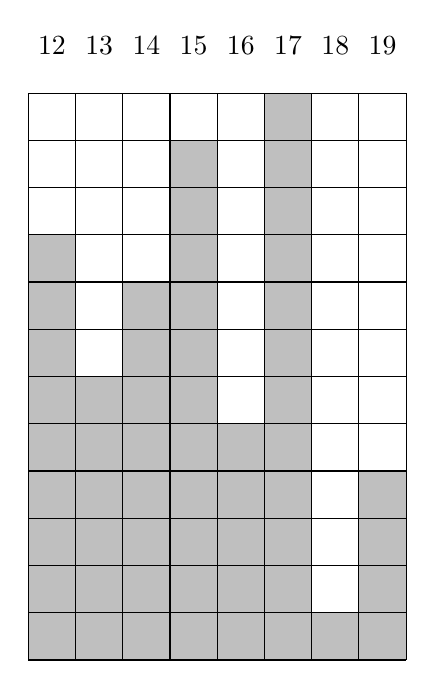
\begin{tikzpicture}[x=6mm,y=6mm]
  % --- Celdas negras ---
  \foreach \x/\y in {%
    5/11,
    5/10, 3/10,
    5/9, 3/9,
    5/8, 3/8, 0/8,
    5/7, 3/7, 0/7, 2/7,
    5/6, 3/6, 0/6, 2/6,
    5/5, 3/5, 0/5, 2/5,1/5,
    5/4, 3/4, 0/4, 2/4,1/4,4/4,
    5/3, 3/3, 0/3, 2/3,1/3,4/3,7/3,
    5/2, 3/2, 0/2, 2/2,1/2,4/2,7/2,
    5/1, 3/1, 0/1, 2/1,1/1,4/1,7/1,
    5/0, 3/0, 0/0, 2/0,1/0,4/0,7/0,6/0,
  }{
   \fill[\CellFill] (\x,\y) rectangle ++(1,1);
  }
\foreach \x/\n in {0/12,1/13,2/14,3/15,4/16,5/17,6/18,7/19}
{
    \node at (0.5+\x,13) {\n};
}

  % --- Rejilla ---
  \draw[step=1, thin] (0,0) grid (\Cols,\Rows);
\end{tikzpicture}
\label{fig: 6-admissible filling sequences}
\caption{An admissible filling sequence}
\end{figure}
\end{example}

We now associate to each admissible filling sequence a composition of operators. 

\begin{definition}\rm \label{def: good pair weights}
Let $\alpha_{i,j}\in \Phi^{\geq 3}$ and  $h=j-i+1$. 
Let $F=(f_0,f_1,\ldots , f_{\ell})$ be an admissible filling sequence.
We define the operator $X_F=X_{\ell-1}\cdots X_{1}$, where each operator $X_s$ is given as follows.
Let $L(f_s)$ be the leftmost white rectangle in $f_s$, $l_s$ be the number of squares in $L(f_s)$, $a_s$  be the label of the leftmost square in $L(f_s)$ and $b_s$  be the label of the rightmost square in $L(f_s)$. 
Then, we define
\begin{itemize}
    \item If $f_{s-1}=f_{s}$ then $X_s = v_{b_s,h}^{l_s}$.
     \item If $f_{s-1}\neq f_{s}$, $ a_{s-1}\neq b_{s-1}$ and $a_s=a_{s-1}$ then $X_s= v_{b_s,h}^{l_s}$.
    \item Otherwise, we set $X_{s}$ equal to the identity operator.  
\end{itemize}
\end{definition}

\begin{example}\rm
    With the same notation as in \Cref{exa: filling sequence} we have
    \begin{equation}
        X_F =    v_{18,10}^1 \circ  v_{18,10}^1 \circ v_{18,10}^1 \circ I\circ I\circ v_{13,10}^1\circ  v_{13,10}^1 \circ I\circ v_{14,10}^3 \circ v_{14,10}^3 . 
    \end{equation}
\end{example}



\begin{lemma}\rm\label{lem: pre - positivo caso bueno}
    Let  $\alpha_{i,j}\in \Phi^{\geq 3}$ and $h=j-i+1$. 
    Let $1\leq k \leq h-2$ and $Y = \Phi^{\succ \alpha_{i,j}}\cup \{ \alpha_{i-k,j-k}  \}$.
    Let $\lambda \in X^+$ be such that $\pint{\lambda }{\alpha_{t}}=0$ for all $t\in [j-k+1,j]$. 
    Then, for all  $B\subset [\alpha_{i-k+1,j-k+1},\alpha_{i,j}]\coloneqq I$, we have
    \begin{equation} \label{eq: pareja buena es positiva}
        \bfM_{\lambda}^{Y\cup B}= \sum_{F\in \mathcal{F}_k(\alpha_{i,j},B)} q^{D(X_F)(\lambda)} \bfM_{X_F(\lambda)}^{\succeq \alpha_{i-k,j-k}}. 
    \end{equation}
    Here, we identify a set $B\subset I$ with the coloring given by the rule that a square in position $j-k+1 \leq s \leq j$ is gray if and only if $\alpha_{s-h+1,s} \in B$.  
    Furthermore, the $\bfM$-elements in \eqref{eq: pareja buena es positiva} indexed by weights for which they are not defined are omitted. 
\end{lemma}

\begin{proof}  
   We proceed by downward induction on the size of the set $B\subset I$. 
   If $B=I$, then $Y\cup B = \Phi^{\succeq \alpha_{i-k,j-k}}$ and $\mathcal{F}_{k}(\alpha_{i,j},B)$ consists of a single filling sequence $\{F\}$ such that $X_F$ is the identity operator. 
   Therefore, there is nothing to prove. 
   
   We now fix $B\subset I$ with $|B|<|I|$ and assume that \cref{eq: pareja buena es positiva} holds for all $B_1\subset I$ with $|B|<|B_1|$ and all $\mu \in X^+$ satisfying $\pint{\mu}{\alpha_t}=0$ for all $t\in [j-k+1,j]$. 
   
   For this $B$, we define $a$ and $b$ as in \eqref{eq: defin a ,b , mu}.  
   We also define $J=[\alpha_{a-h+1,a}, \alpha_{b-h,b-1}]$.
   We note that, under the identification described in the statement, the set $J\subset B$ corresponds to the leftmost white region of $B$. 

   For $a\leq c \leq b-1$, we define
   \[
      A_c= Y\cup B \cup \{\alpha_{c-h+1,c}\}
      \qquad\text{and}\qquad
      J_c= [\alpha_{a-h+1,a}, \alpha_{c-h,c-1}].
   \]
   
   By the definition of the $\bfM$-elements, we have
 \begin{equation}  \label{eq: desc subintervalos}
    \bfM_{\lambda}^{Y\cup B} =   \bfM_{\lambda}^{A_a} +     \sum_{c=a+1}^{b-1} 
    q^{c-a}\bfM_{\lambda - \Sigma_{J_c} }^{A_{c} } +q^{b-a}\bfM_{\lambda-\Sigma_{J}}^{Y\cup B}  .
 \end{equation}
 
 Applying \Cref{lem: lamda - alpha  a v}, we obtain
 \begin{equation}  \label{eq: desc subintervalos dominantes}
    \bfM_{\lambda}^{Y\cup B} = 
    \bfM_{\lambda}^{A_a} +  \sum_{c=a+1}^{b-1} q^{D(v_{c-1,h}^{c-a})(\lambda)}\bfM_{v_{c-1,h}^{c-a}(\lambda)}^{A_{c}}  + 
    q^{D(v_{b-1,h}^{b-a})(\lambda )}\bfM_{v_{b-1,h}^{b-a}(\lambda )}^{Y\cup B}. 
 \end{equation}

Since $|Y\cup B|<|A_c|$ for all $a\leq c \leq b-1$, we may apply our inductive hypothesis to rewrite all terms indexed by the sets $A_c$ using \cref{eq: pareja buena es positiva}. 

Although the last term on the right-hand side of \cref{eq: desc subintervalos dominantes} is not covered by the downward induction on $|B|$, we can still apply \cref{eq: pareja buena es positiva} to it because $v_{b-1,h}^{b-a}(\lambda )< \lambda$, and hence we may invoke induction on the dominance order. 

The result then follows from the definition of admissible filling sequences and the operators associated with them. Namely, if
\[
F =(f_0,f_1, ..,f_{\ell})\in \mathcal{F}_k(\alpha_{i,j}, B),
\]
then, under the identification described in the statement, we must have either $f_1=\emptyset$ or $f_1=A_c$ for some $a\leq c \leq b-1$. 
Therefore, we obtain the following disjoint decomposition:
\begin{equation}
    \mathcal{F}(\alpha_{i,j},B) = \mathcal{F}(\alpha_{i,j},B)_{\emptyset} \cup \bigcup_{c=a}^{b-1} \mathcal{F}(\alpha_{i,j},B)_{A_c},  
\end{equation}
where
\[
\mathcal{F}(\alpha_{i,j},B)_{S}
=
\{ F\in \mathcal{F}(\alpha_{i,j},B) \mid f_1=S  \}.
\]
The claim now follows.
\end{proof}




\begin{proposition}\rm \label{prop: caso bueno}
 Let $\lambda \in X^{+}$, $\alpha_{i,j}\in \Phi^{\geq 3}$ and  $h=j-i+1$. 
    Let $1\leq k < h-1$ and suppose that $ \pint{\lambda}{\alpha_{t}} =0$ for $t\in [j-k+1,j]$. 
    Furthermore, we assume that $\mu_k\coloneqq v^k_{j,h}(\lambda) $ is defined.
    Then, we have
    \begin{equation} \label{sumsum}
        \bfM_{\mu_k}^{\succ \alpha_{i,j}} - q\bfM_{\mu_k - \alpha_{i-k,j-k}}^{\succ \alpha_{i,j}} =  \sum_{F\in \mathcal{F}_k(\alpha_{i,j},\emptyset)} q^{D(X_F)(\mu_k)}\bfM_{X_F(\mu_k)}^{ \succeq \alpha_{i-k,j-k}   }, 
    \end{equation}   
    where $\bfM$-elements indexed by undefined weights are neglected. 
\end{proposition}

\begin{proof}
    By the conditions imposed on $\lambda$ we have that $\mu_k$ satisfies the conditions in \Cref{lem: pre - positivo caso bueno}. 
    On the other hand, if $Y=\Phi^{\alpha_{i,j}}\cup \{\alpha_{i-k,j-k}\}$ then we have
    \begin{equation}
        \bfM_{\mu_{k}}^Y  = \bfM_{\mu_k}^{\succ \alpha_{i,j}} - q\bfM_{\mu_k - \alpha_{i-k,j-k}}^{\succ \alpha_{i,j}} . 
    \end{equation}
    Therefore, the result follows by applying \Cref{lem: pre - positivo caso bueno} for $B=\emptyset$. 
\end{proof}


\begin{example}\rm
Figure \ref{fig:rectangles} depicts the nine admissible filling sequences that contribute to the expansion of the element $X_3$ in \Cref{ex: como funciona}, as predicted by \Cref{prop: caso bueno}.
The weight associated with each filling sequence is displayed below the corresponding diagram.

Although there are infinitely many admissible filling sequences, only finitely many contribute to the expansion in \eqref{sumsum}.
\end{example}


\begin{figure}[ht]
\centering

\newcommand{\rectcell}[2]{%
\begin{minipage}{0.28\textwidth}
\centering
#1

\vspace{2mm}
$#2$
\end{minipage}%
}

\rectcell{\grayrect[4]{1/6,1/7,1/8,2/6,2/7,3/6}}{\mu}
\hfill
\rectcell{\grayrect{1/6,1/7,1/8,2/6,2/7,3/6}}{v_{8,5}^{3}(\mu)}
\hfill
\rectcell{\grayrect{1/6,1/7,1/8,2/6,2/8,3/6}}{v_{7,5}^{1}v_{8,5}^{3}(\mu)}


\vspace{4mm}

\rectcell{\grayrect[5]{1/6,1/7,1/8,2/6,2/8,3/8}}
{v_{7,5}^{2}v_{8,5}^{3}(\mu)}
\hfill
\rectcell{\grayrect{1/6,1/7,1/8,2/6,2/7,3/6,4/6}}{v_{8,5}^{2}(\mu)}
\hfill
\rectcell{\grayrect{1/6,1/7,1/8,2/6,2/8,3/6,4/6}}
{v_{7,5}^{1}v_{8,5}^{2}(\mu)}


\vspace{4mm}

\rectcell{\grayrect{1/6,1/7,1/8,2/6,2/7,3/6,3/7,4/6}}{v_{8,5}^{1}(\mu)}
\hfill
\rectcell{\grayrect[4]{1/6,1/7,1/8,2/6,2/8,3/6}}{v_{7,5}^{1}(\mu)}
\hfill
\rectcell{\grayrect[4]{1/6,1/7,1/8,2/6,2/8,3/8}}{v_{7,5}^{2}(\mu)}

\caption{Filling sequences of rectangles and their corresponding weights}
\label{fig:rectangles}
\end{figure}



%%%%%%%%%%%%%%%%%%%%%%%%%%%%%%%%%%%%%%%%%%%%%%%%%%%%%%%%%%%%%%%%%

\subsection{Commutation Rules} \label{section COM RUl}

Having established in the previous section that good pairs expand positively, we now turn our attention to the bad pair appearing in the SID.

To handle this case, we require a collection of commutation rules between the relevant operators. The main purpose of this section is to state these rules.

For the sake of brevity, we omit their proofs. The arguments consist of a lengthy case-by-case analysis that, while technical, offers little additional insight into the underlying ideas. Instead, we present several examples that illustrate the rules and provide intuition for why they hold.

We emphasize that the commutation rules stated below do not apply to arbitrary dominant weights. Rather, they are valid only for a special class of dominant weights satisfying an additional condition.


% \vspace{2cm}
% %-----------------
% %COMENTARIO
% %-----------------
% En principio, la conmutación que queremos al ser cada lado formada por una secuencia consecutiva de P operadores, siempre la existencia del siguiente operador vendrá asegurada por el anterior ($...P_sP_{s+1}...$), esto tambien acota las posibilidades de $\varrho_s$ en cada paso, pues por la desigualdad de $\varrho$'s, siempre tendremos una cota inferior, además como a medida que nos acercamos al final de un $\mathbf{P}$ los largos de los operadores se hacen cada vez mas cortos, entonces las posibilidades de varrhos se vuelven más y más acotadas hasta que la misma estructura de los P operadores los hace colapsar en una igualdad.

% Esa explicación anterior tiene sentido siempre y cuando estamos hablando de $P_s$ a los cuales se les realizó un $P_{s+1}$ justo antes, el caso complejo viene cuando estamos en $P_{i}$. Cómo $P_i$ no tiene ningún operador antes, su existencia no depende de otros, por lo cual al anteponer un operador, por ejemplo $P_{i+1}$, el cual afecta directamente al $\varrho_i$, puede provocar que el operador cambie, dependiendo de si $P_{i+1}$ está antes o despues de él.

% Por ejemplo, si $P_{i+1}$ está despues de él y estamos en altura 3 o más, entonces $P_{i+1}$ no recibe ninguna restricción provocada por $P_{i}$, mientras que $P_{i}$ es completamente independiente de $P_{i+1}$, básicamente porque fue hecho antes.
% Por otro lado, si $P_{i+1}$ es hecho primero, entonces este nuevamente es completamente independiente de $P_i$, porque está hecho antes, pero en este caso, $P_i$ podría ser afectado por $P_{i+1}$, provocando que su $\varrho_i$ cambie.

% Aquí es donde entra la condición $Z$. La idea de esta condición es asegurar la independencia del $P_{i}$ con el $P_{i+1}$. El caso que arruina la conmutación es cuando $\varrho_{i+1}>\varrho_{i}+h$, esto pues puede otorgar un 1 a una posición congruente a $i-h+1$, pero más alta, esto provocará que la elección de $\varrho_{i}$ cambie y por lo tanto cambie completamente el peso.

% La condición $Z$ Asegura que siempre hay 0 por arriba de $\varrho_{i}+h$, provocando que el caso anterior sea imposible, en teoría si solo conmutara $P_{i+1}$ podría pedir una condición Z más debil, como por ejemplo solamente 0 en las posiciones congruentes a $i-h+2$, pero como estamos conmutando $P_{i+1}P_{i+2} \cdots $, entonces si cualquiera de esos operadores mayores tuviera su $\varrho$ mayor de $\varrho_{i}+h$ entonces otorgaría al que sigue una posición mayor, lo que finalmente haría que se le otorgara a $P_{i+1}$ rompiendo la conmutación.

% En el caso de la conmutación en lemma 7.16, esto no es un problema, porque lo que deseamos conmutar es un $X_Fv_{j_s}^m$ y en esencia cada uno de esos $X_f$ que forman el $X_F$ y tambien el $v_{j_s}^m$ están compuestos por secuencias de $P$ operadores, donde el índice más pequeño que tienen es a lo menos i+2, nunca habrá un $P_{i+1}$ molestando al $P_i$ como en el caso anterior. Esto implica que no necesito toda la condición Z, solamente necesito los 0 que hacen que $v_{j_s}^m$ y $X_F$ tengan sentido.








\begin{definition}\rm
Let $\alpha_{i,j} \in \Phi^{\geq 2}$ and set $h = j-i+1$. We say that a dominant weight $\lambda$ satisfies Condition $\mathbf{Z}$ if $P_{i,h}(\lambda)$ is defined and, setting $\varrho \coloneq \varrho_{i,h}(\lambda)$, we have
$$ \pint{\lambda}{\alpha_t} = 0 \quad \text{for all integers } t \in [\varrho+h, j]. $$
\end{definition}



\begin{lemma}\label{lem: super-conmutation}
Let $\lambda \in X^+$, $\alpha_{i,j}\in \Phi^{\geq 2}$, and  $h=j-i+1$. 
Let $s$ be an integer such that $0\leq s\leq h-2$, and define $j_s\coloneqq j-s$. 
Assume that $\lambda$ satisfies Condition $\mathbf{Z}$ and that the weight
$\mathbf{P}_{j_s,h}\mathbf{P}_{i,h}(\lambda)$ is defined.
Then $\mathbf{P}_{j_s,h}(\lambda)$ is also defined, and
\begin{equation}\label{eq: super-commutation}
    \mathbf{P}_{j_s,h}(\lambda)
    =
    \mathbf{P}_{j_s,h}\mathbf{P}_{i,h}(\lambda).
\end{equation}
\end{lemma}


\begin{example}\label{exa:  conmutation}  \rm
In this example we illustrate  \Cref{lem: super-conmutation}.

Let us fix the parameters $(i, j) = (9, 11)$ and $h = 11 - 9 + 1 = 3$. According to the lemma, the integer $s$ can take values in the range $0 \le s \le h-2$, which gives $s \in \{0, 1\}$. 
Thus, the relevant indices are $j_0 = 11$ and $j_1 = 10$. 
Let
\[
    \lambda = [6, 2, 1, 1, 2, 0, 0, 0, 0, 0, 0, 1]_\varpi.
\]
We have
\begin{equation}
    P_{9,3}(\lambda) = \lambda - \alpha_{4,9} = [6, 3, 0, 1, 2, 0, 0, 0, -1, 1, 0, 1]_\varpi .
\end{equation}
In particular,  $\varrho_{9,3}(\lambda) = 4$. 
Therefore, $\lambda$ satisfies Condition $\mathbf{Z}$ since $\pint{\lambda}{\alpha_k} =0$ for all integers $k\in [7,11]$. 
We want to  verify \eqref{eq: super-commutation} for $j_0=11$ and $j_1=11$. 
For $j_0=11$ we have 
\begin{equation}
\begin{aligned}
    \mathbf{P}_{9,3}(\lambda) &= \lambda - \alpha_{4,9} - \alpha_{3,8} - \alpha_{5,7} - \alpha_{4,6} - \alpha_{3,5} \\
    &= [6, 4, 1, 0, 0, 0, 0, 0, 0, 1, 0, 1]_\varpi, \\[5pt]
    \mathbf{P}_{11,3}\mathbf{P}_{9,3}(\lambda) &= \mathbf{P}_{9,3}(\lambda) - \alpha_{3,11} - \alpha_{2,10} \\
    &= [7, 4, 0, 0, 0, 0, 0, 0, 0, 0, 0, 2]_\varpi.
\end{aligned}
\end{equation}
On the other hand, applying $\mathbf{P}_{11,3}$ directly to $\lambda$ yields:
\begin{equation}
\begin{aligned}
    \mathbf{P}_{11,3}(\lambda) &= \lambda - \alpha_{3,11} - \alpha_{5,10} - \alpha_{4,9} -\alpha_{3,8} - \alpha_{5,7} - \alpha_{4,6} - \alpha_{3,5} - \alpha_{2,4} \\
    &= [7, 4, 0, 0, 0, 0, 0, 0, 0, 0, 0, 2]_\varpi \\
    & = \mathbf{P}_{11,3}\mathbf{P}_{9,3}(\lambda).
\end{aligned}
\end{equation}
Similarly, for $j_1 = 10$ we have
\begin{equation}
\begin{aligned}
    \mathbf{P}_{10,3}\mathbf{P}_{9,3}(\lambda) &= \mathbf{P}_{9,3}(\lambda) - \alpha_{2,10} \\
    &= [7, 3, 1, 0, 0, 0, 0, 0, 0, 0, 1, 1]_\varpi, \\[5pt]
    \mathbf{P}_{10,3}(\lambda) &= \lambda - \alpha_{5,10} - \alpha_{4,9} - \alpha_{3,8} - \alpha_{5,7} - \alpha_{4,6}- \alpha_{3,5} - \alpha_{2,4} \\
    &= [7, 3, 1, 0, 0, 0, 0, 0, 0, 0, 1, 1]_\varpi \\ &= \mathbf{P}_{10,3}\mathbf{P}_{9,3}(\lambda).
\end{aligned}
\end{equation}
In both instances, the equality $\mathbf{P}_{j_s, 3}\mathbf{P}_{9,3}(\lambda) = \mathbf{P}_{j_s, 3}(\lambda)$ predicted by the lemma holds. 
\end{example}



\begin{example}\rm
Consider the same parameters as in \Cref{exa:  conmutation} but  the weight 
\[
    \lambda = [6, 2, 3, 0, 2, 1, 0, 0, 0, 0, 0, 1]_{\varpi}.
\]
We have $P_{9,3}(\lambda) = \lambda - \alpha_{1,9} = [5, 2, 3, 0, 2, 1, 0, 0, -1, 1, 0, 1]_{\varpi}$.
In particular, $\varrho_{9,3}(\lambda)=1$. 
Thus,  Condition $\mathbf{Z}$ requires $\langle \lambda, \alpha_t \rangle = 0$ for all $t \in  [4, 11]$. 
Since  $\pint{\lambda}{\alpha_5} = 2\neq 0$, we have that $\lambda$ does not satisfy Condition $\mathbf{Z}$. 

Let us show that \eqref{eq: super-commutation} does not hold in this case. 
We first notice that

\begin{equation}
\begin{aligned}
    \mathbf{P}_{9,3}(\lambda) &= \lambda - \alpha_{1,9}- \alpha_{6,8}- \alpha_{5,7}- \alpha_{4,6}- \alpha_{3,5} \\
    &= [5, 3, 3, 0, 1, 0, 0, 0, 0, 1, 0, 1]_\varpi.
\end{aligned}
\end{equation}

Therefore, we get
\begin{equation}
\begin{aligned}
    \mathbf{P}_{10,3}\mathbf{P}_{9,3}(\lambda) &= \mathbf{P}_{9,3}(\lambda)- \alpha_{5,10} \\
    &= [5, 3, 3, 1, 0, 0, 0, 0, 0, 0, 1, 1]_\varpi.
\end{aligned}
\end{equation}
On the other hand, we have
\begin{equation}
    \begin{aligned}
         \mathbf{P}_{10,3}(\lambda) &= \lambda- \alpha_{5,10} - \alpha_{4,9}- \alpha_{6,8}- \alpha_{5,7}- \alpha_{4,6}- \alpha_{3,5} \\
    &= [6, 3, 4, 0, 0, 0, 0, 0, 0, 0, 1, 1]_\varpi.
    \end{aligned}
\end{equation}
We conclude that 
$   \mathbf{P}_{10,3}\mathbf{P}_{9,3}(\lambda) \neq \mathbf{P}_{10,3}(\lambda)$. 
Thus \eqref{eq: super-commutation} fails for $j_1=10$. 
\end{example}




\begin{lemma}\rm\label{conm. 2}
Let $\alpha_{i,j} \in \Phi^{\geq 3}$ and set $h = j-i+1$. 
Let $s$ and $m$ be integers satisfying $0 \leq s < h-2$ and $1 \leq m \leq h-2-s$. 
Define $j_s = j-s$ and $i_s = i-s$. 
Let $F \in \mathcal{F}_m(\alpha_{i_s,j_s},B)$, where $B$ is the coloring in which all boxes are white, and let $X_F$ denote its corresponding operator. 
Suppose $\lambda \in X^{+}$ is such that $\pint{\lambda}{\alpha_{t}} = 0$ for all $t \in [i+1,j]$. 
If $X_F(v_{j_s,h}^m\mathbf{P}_{i,h}(\lambda))$ is defined, then $\mathbf{P}_{i,h}(X_F v_{j_s,h}^m(\lambda))$ is also defined, and the following equality holds:
\begin{equation}\label{eq: conm. 2}
    X_{F}(v_{j_s,h}^{m}\mathbf{P}_{i,h}(\lambda)) = \mathbf{P}_{i,h}(X_{F} v_{j_s,h}^m(\lambda)).
\end{equation}
\end{lemma}

%-------------------------------
%ENUNCIADO ANTERIOR
%-------------------------------

% \begin{lemma}\label{conm. 2}
%     Let $\lambda\in X^+$, $\alpha_{i,j} \in \Phi^{\geq 3}$, $h = j-i+1$, and $(s,m)$ be a pair integers satisfying  $0\leq s < h-2$, $1 \leq m \leq h-2-s$.
%     Set $j_s = j-s$.
%     Let $\mathcal{F}_m$ denote the set of $m$-fillings whose rightmost empty box is labeled by $j_s-m$. 
%     If $\lambda$ satisfies the condition Z, then
%     for any $F \in \mathcal{F}_m$ such that 
%     $X_{F}(v_{j_s,h}^{m}\mathbf{P}_{i,h}(\lambda))$
%     is defined, the following identity holds:
%     \begin{equation}\label{eq: conm. 2}
%          X_{F}(v_{j_s,h}^{m}\mathbf{P}_{i,h}(\lambda)) = \mathbf{P}_{i,h}(X_{F} \, v_{j_s,h}^m(\lambda)).
%     \end{equation}
% \end{lemma}




\begin{example}\rm
In this example, we illustrate the commutation relation described in \Cref{conm. 2}.

Let us fix the parameter $\alpha_{i,j} = \alpha_{11,14}$, $h = j-i+1 = 4$ and consider the operator $\mathbf{P}_{11,4}$. 
We will examine its commutation with the sequence of operators $X_F(v^{2}_{14,4}) = (v^1_{13,4})^3(v^{2}_{14,4})^2$.
This sequence arises from the $2$-filling illustrated in the following figure:

\begin{figure}[H]
\centering
\def\Cols{2}
\def\Rows{6}
% Cambia este valor: gray!70 = más oscuro, gray!40 = más claro
\def\CellFill{gray!50}
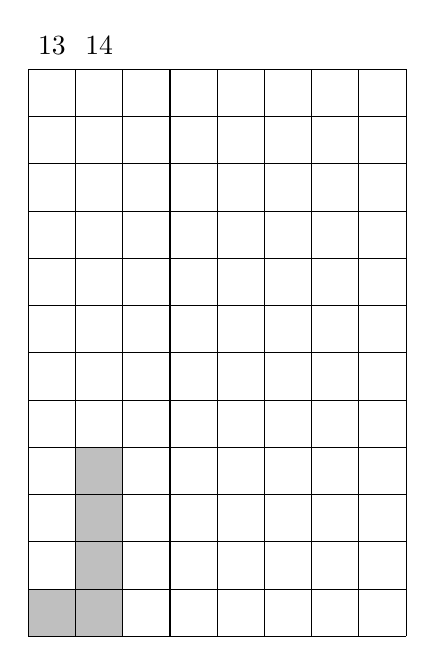
\begin{tikzpicture}[x=6mm,y=6mm]
  % --- Celdas negras ---
  \foreach \x/\y in {%
    1/3,
    1/2,
    1/1,
    0/0,1/0
  }{
   \fill[\CellFill] (\x,\y) rectangle ++(1,1);
  }
    \foreach \x/\n in {0/13,1/14}
    {
        \node at (0.5+\x,\Rows + 0.5) {\n};
    }
  % --- Rejilla ---
  \draw[step=1, thin] (0,0) grid (\Cols,\Rows);
\end{tikzpicture}
\caption{2-admissible filling sequences}
\label{fig: 2-admissible filling sequences}
\end{figure}

Consider the following weight:
\[
    \lambda = [3, 3, 2, 3, 3, 2, 0, 0, 0, 0, 0, 0, 0, 0, 2, 2, 0, 1, 5, 0]_\varpi.
\]

\medskip
\noindent First, we apply the composite operator $(v^1_{13,4})^3(v^{2}_{14,4})^2\mathbf{P}_{11,4}$ to $\lambda$:
\begin{equation}
\begin{aligned}
    \mathbf{P}_{11,4}(\lambda) &= \lambda - \alpha_{4,11} - \alpha_{3,10} - \alpha_{6,9} - \alpha_{5,8} - \alpha_{3,6} \\
    &= [3, 5, 2, 2, 3, 0, 0, 0, 0, 0, 0, 1, 0, 0, 2, 2, 0, 1, 5, 0]_\varpi, \\[5pt]
    v^{2}_{14,4}\mathbf{P}_{11,4}(\lambda) &= \mathbf{P}_{11,4}(\lambda) - \alpha_{3,17}- \alpha_{2,16} \\
    &= [4, 5, 1, 2, 3, 0, 0, 0, 0, 0, 0, 1, 0, 0, 2, 1, 0, 2, 5, 0]_\varpi, \\[5pt]
    (v^1_{13,4})^3(v^{2}_{14,4})^2\mathbf{P}_{11,4}(\lambda) &= v^{2}_{14,4}\mathbf{P}_{11,4}(\lambda) - \alpha_{3,17}- \alpha_{2,16}- 3\alpha_{2,19} \\
    &= [8, 2, 0, 2, 3, 0, 0, 0, 0, 0, 0, 1, 0, 0, 2, 0, 0, 3, 2, 3]_\varpi.
\end{aligned}
\end{equation}

\medskip
\noindent Next, we reverse the order: we apply the sequence of $v$-operators to the initial weight $\lambda$ first, followed by the $\mathbf{P}$-operator (i.e., we evaluate $\mathbf{P}_{11,4}(v^1_{13,4})^3(v^{2}_{14,4})^2(\lambda)$):
\begin{equation}
\begin{aligned}
    (v^1_{13,4})^3(v^{2}_{14,4})^2(\lambda) &= \lambda - 2\alpha_{3,17}- 2\alpha_{6,16}- 3\alpha_{2,19} \\
    &= [6, 2, 0, 3, 5, 0, 0, 0, 0, 0, 0, 0, 0, 0, 2, 0, 0, 3, 2, 3]_\varpi, \\[5pt]
    \mathbf{P}_{11,4}\Big((v^1_{13,4})^3(v^{2}_{14,4})^2(\lambda)\Big) &= (v^1_{13,4})^3(v^{2}_{14,4})^2(\lambda) - \alpha_{4,11} - \alpha_{3,10} - \alpha_{2,9}  - \alpha_{5,8} - \alpha_{4,7} - \alpha_{3,6} - \alpha_{2,5} \\
    &= [8, 2, 0, 2, 3, 0, 0, 0, 0, 0, 0, 1, 0, 0, 2, 0, 0, 3, 2, 3]_\varpi.
\end{aligned}
\end{equation}

Therefore, 
\[
    (v^1_{13,4})^3(v^{2}_{14,4})^2\mathbf{P}_{11,4}(\lambda) = \mathbf{P}_{11,4}(v^1_{13,4})^3(v^{2}_{14,4})^2(\lambda).
\] 
\end{example}
% Furthermore, observe that the intermediate weight 
% $$\mu = (v^1_{13,4})^3(v^{2}_{14,4})^2(\lambda) = [6, 2, 0, 3, 5, 0, 0, 0, 0, 0, 0, 0, 0, 0, 2, 0, 0, 3, 2, 3]_\varpi$$
% strictly satisfies Condition $\mathbf{Z}$, since $\varrho_{14,4}(\mu) = 4$ and $\mu_{8} = \mu_{9} = \mu_{10} = \mu_{11} = \mu_{12} = \mu_{13} = \mu_{14} = 0$.


\subsection{Proof of positivity}  \label{section proof of positivity}

The following lemma will allow us to handle the case when a bad pair occurs in the Second Inverse Decomosition. 

\begin{lemma} \label{lem: GranLemma}
    Let $\alpha_{i,j} \in \Phi^{\geq 2} $ and  $h=j-i+1$.
    For $\lambda \in X^{+}$ we define
    \begin{equation}
       \mathcal{A}_\lambda^{i,j} \coloneqq \sum_{\mu< \lambda}  \mathbb{N}[q] \bfM_{\mu}^{\succ\alpha_{i,j}}+
         \sum_{t=0}^{i-1} \left( \sum_{\substack{\mu \in X^+ \\\mu\leq  \lambda}}\mathbb{N}[q]\bfM_{\mu}^{\succeq \alpha_{i-t,j-t}} \right). 
    \end{equation}
If  $\lambda$ satisfies Condition $Z$ and  $\mathbf{P}_{i,h}(\lambda)$ is defined then
\begin{equation} \label{eq: DIFF}
    \bfM_{\lambda}^{\succ \alpha_{i-s,j-s}} - q^{D(\mathbf{P}_{i,h} )(\lambda)}  \bfM_{\mathbf{P}_{i,h}(\lambda)}^{\succ \alpha_{i-s,j-s}} \in  \mathcal{A}_\lambda^{i,j},
\end{equation}
for all $ 0\leq s \leq h-1  $. 
\end{lemma}



\begin{proof}
We proceed by induction on $i$. 
We notice that if $i<h$, then $i-h+1<1$.
Thus, the root $\alpha_{i-h+1,i}$ is not defined. 
It follows that $\mathbf{P}_{i,h}(\lambda)$ is not defined.
Therefore, we must have $i\geq h$, and the base case of our induction is the case $i=h$. 


For $0\leq s \leq h-1$ we set $i_s=i-s$ and $j_{s}=j-s$. 
    
By combining \Cref{prop: second version refinado} and \Cref{prop: caso bueno}, we obtain
        \begin{equation}\label{eq:super-lemma-A}
        \bfM_{\lambda}^{\succ \alpha_{i_s,j_s}} =   \bfM_{\lambda}^{\succeq \alpha_{i_s,j_s}} +q^{D(\mathbf{P}_{j_s,h})(\lambda)} \bfM_{ \mathbf{P}_{j_s,h}(\lambda )}^{\succ \alpha_{i_s,j_s}} + \sum_{m=1}^{h-2}  q^{D(v_{j_s,h}^m)(\lambda)}  X_m + q^{D(\mathbf{v}_{j,h})(\lambda)}Y_s,
    \end{equation}
where 
\begin{equation}\label{eq: XXX}
    X_m = \displaystyle\sum_{F\in \mathcal{F}_m} q^{D(X_F)(v_{j_s,h}^m(\lambda))} \mathbf{M}_{X_F(v_{j_s,h}^m(\lambda))}^{\succeq \alpha_{i_s-m,j_s-m}}.
\end{equation}
and 
\begin{equation}\label{eq: YsubS}
    Y_s=  \bfM_{\mathbf{v}_{j_s,h}(\lambda )}^{\succ \alpha_{i_s,j_s}}-q^{D(\mathbf{P}_{i_s,h})(\mathbf{v}_{j_s,h}(\lambda ))}\bfM_{\mathbf{P}_{i_s,h}\mathbf{v}_{j_s,h}(\lambda )}^{\succ \alpha_{i_s,j_s}}.  
\end{equation}


On the other hand, we notice that $\pint{\mathbf{P}_{i,h}(\lambda)}{\alpha_{i+1}} = 1$ and $\pint{\mathbf{P}_{i,h}(\lambda)}{\alpha_{t}} = 0$ for all $t \in [i+2, j]$. 
Thus, \Cref{prop: second version refinado} and \Cref{prop: caso bueno} yield
\begin{equation} \label{eq: M de P_i}
     \mathbf{M}_{\mathbf{P}_{i,h}(\lambda)}^{\succ \alpha_{i_s ,j_s}} = \mathbf{M}_{\mathbf{P}_{i,h}(\lambda)}^{\succeq \alpha_{i_s ,j_s}} +  q^{D(\mathbf{P}_{j_s,h})(\mathbf{P}_{i,h}(\lambda))}\mathbf{M}_{\mathbf{P}_{j_s,h}\mathbf{P}_{i,h}(\lambda)}^{\succ \alpha_{i_s ,j_s}} + \sum_{m=1}^{h-2-s}q^{D(v_{j_s,h}^m)(\mathbf{P}_{i,h}(\lambda))}X'_m,
\end{equation}
where 
\begin{equation}\label{eq: XXX prime}
    X'_m =  \sum_{F\in \mathcal{F}_m} q^{D(X_F)(v_{j_s,h}^m(\mathbf{P}_{i,h}(\lambda)))} \mathbf{M}_{X_F(v_{j_s,h}^m(\mathbf{P}_{i,h}(\lambda)))}^{\succeq \alpha_{i_s-m,j_s-m}}.
\end{equation}

We insist on our convention that if a weight $\mu$ is not defined, then the corresponding $\bfM$-term is set equal to zero.
In order to save space, we set
\begin{equation}
    \Delta_\lambda^{i}(s) \coloneqq   \bfM_{\lambda}^{\succ \alpha_{i-s,j-s}} - q^{D(\mathbf{P}_{i,h} )(\lambda)}  \bfM_{\mathbf{P}_{i,h}(\lambda)}^{\succ \alpha_{i-s,j-s}}. 
\end{equation}


We first treat the base case $i=h$. 
We split the proof into three cases.

\begin{itemize}
    \item $s=h-1$.  We have $j_s=j-(h-1)=i$. Therefore, by \eqref{eq:super-lemma-A} we have
    \begin{equation}
\Delta_{\lambda}^i(s)  =   \bfM_{\lambda}^{\succeq \alpha_{i_s,j_s}}  + \sum_{m=1}^{h-2}  q^{D(v_{j_s,h}^m)(\lambda)}  X_m + q^{D(\mathbf{v}_{j,h})(\lambda)}Y_s.  
    \end{equation}
By \eqref{eq: XXX} we know that $X_m\in \mathcal{A}_{\lambda}^{i,j}$ for all $1\leq m \leq h-2$.  
Thus, we only need to analyze the element $Y_s$. 
We notice that in this case $i_s<i=h$.
By the discussion in the first paragraph of this proof, we conclude that the weight $\mathbf{P}_{i_s,h}\mathbf{v}_{j_s,h}(\lambda )$ is not defined. 
In accordance with our conventions, \eqref{eq: YsubS} reduces to 
\begin{equation}\label{eq: YYY solo}
       Y_s=  \bfM_{\mathbf{v}_{j_s,h}(\lambda )}^{\succ \alpha_{i_s,j_s}}.
\end{equation}
Since $\mathbf{v}_{j_s,h}(\lambda)<\lambda$, it follows that $Y_s\in \mathcal{A}_{\lambda}^{i,j}$. 
Therefore, $\Delta_{\lambda}^i(s) \in  \mathcal{A}_{\lambda}^{i,j}$, as we wanted to show. 

\item $s=h-2$. We combine \eqref{eq:super-lemma-A}
 and \eqref{eq: M de P_i} to compute $\Delta_{\lambda}^i(s)$.
 By using \Cref{lem: super-conmutation}, we get
 \begin{equation}
     \mathbf{P}_{j_s,h}(\lambda) = \mathbf{P}_{j_s,h}\mathbf{P}_{i,h}(\lambda) \qquad \mbox{and} \qquad D(\mathbf{P}_{j_s,h})(\lambda) = D(\mathbf{P}_{i,h})(\lambda) + D(\mathbf{P}_{j_s,h})(\mathbf{P}_{i,h})(\lambda). 
 \end{equation}
 Therefore, the corresponding terms cancel each other in $\Delta_{\lambda}^i(s)$.
 Thus, in this case the lemma reduces to proving that both 
 \begin{equation}
  \bfM_{\lambda}^{\succeq \alpha_{i_s,j_s}} - q^{D(\mathbf{P}_{i,h})(\lambda)} \bfM_{\mathbf{P}_{i,h}(\lambda)}^{\succeq \alpha_{i_s,j_s}}   \qquad \mbox{and} \qquad    Y_s
 \end{equation}
 belong to $\mathcal{A}_{\lambda}^{i,j}$. 

On the one hand, we have
\begin{equation} \label{eq: case h-2}
   \bfM_{\lambda}^{\succeq \alpha_{i_s,j_s}} - q^{D(\mathbf{P}_{i,h})(\lambda)} \bfM_{\mathbf{P}_{i,h}(\lambda)}^{\succeq \alpha_{i_s,j_s}} = \Delta_{\lambda}^i(s+1).  
\end{equation}
The right-hand side of \eqref{eq: case h-2} belongs to $\mathcal{A}_{\lambda}^{i,j}$ by the case $s=h-1$ treated above. 

On the other hand, if $h>2$, then $i_s<i=h$, so we can conclude that $Y_s\in \mathcal{A}_{\lambda}^{i,j}$ by arguing as in the previous case. 
If $h=2$, then $s=0$, so that $Y_s= \Delta_{\mathbf{v}_{j,h}(\lambda)}^i(s)$. 
Since $\mathbf{v}_{j,h}(\lambda) <\lambda$, we can argue by induction on the dominance order to conclude that $Y_s\in \mathcal{A}_{\lambda}^{i,j}$. 


\smallskip
 \item Let $0\leq s < h-2$.
 We argue in the same fashion as in the previous case. 
That is, we combine \eqref{eq:super-lemma-A}
 and \eqref{eq: M de P_i} to compute $\Delta_{\lambda}^i(s)$. 
 After this, we use \Cref{lem: super-conmutation} to cancel the terms indexed by $ \mathbf{P}_{j_s,h}(\lambda) $ and $\mathbf{P}_{j_s,h}\mathbf{P}_{i,h}(\lambda)$. 
 Next, we use downward induction on $s$ to conclude that the difference on the left-hand side of \eqref{eq: case h-2} belongs to $\mathcal{A}_{\lambda}^{i,j}$. 
 Similarly, the term $Y_s$ can be shown to belong to $\mathcal{A}_{\lambda}^{i,j}$ by the same argument as in the previous case, namely: either $Y_s \in \mathcal{A}_{\lambda}^{i,j}$ if $s>0$ by \eqref{eq: YYY solo}, or $Y_s \in \mathcal{A}_{\lambda}^{i,j}$ if $s=0$ by induction on the dominance order. 
 
 All in all, we realize that negative terms in $\Delta_{\lambda}^i(s)$ can only arise from the differences between the $X_m$ and $X_m'$ terms. 
 Concretely, this case reduces to proving that 
\begin{equation}
   q^{D(v_{j_s,h}^m)(\lambda)}  X_m  - q^{D(\mathbf{P}_{i,h})(\lambda)} q^{D(v_{j_s,h}^m)(\mathbf{P}_{i,h}(\lambda))}X'_m \in \mathcal{A}_{\lambda}^{i,j}
\end{equation}
for all $1\leq m \leq h-2-s$. 

By combining \eqref{eq: XXX} and \eqref{eq: XXX prime}, together with the additivity of the degrees, it is enough to prove that  
\begin{equation} \label{eq: it is enough A}
   q^{D(X_F\, v_{j_s,h}^m)(\lambda)}  \mathbf{M}_{X_F(v_{j_s,h}^m(\lambda))}^{\succeq \alpha_{i_s-m,j_s-m}}  - q^{D(X_F\, v_{j_s,h}^m \mathbf{P}_{i,h})(\lambda)} \mathbf{M}_{X_F(v_{j_s,h}^m(\mathbf{P}_{i,h}(\lambda)))}^{\succeq \alpha_{i_s-m,j_s-m}}\in \mathcal{A}_{\lambda}^{i,j},
\end{equation}
for all $1\leq m \leq h-2-s$. 

If $X_F(v_{j_s,h}^m(\mathbf{P}_{i,h}(\lambda)))$ is not defined, then we are done by our conventions. 
Otherwise, by \Cref{conm. 2} we have that
\begin{equation}\label{eq: XXX conm}
    X_F(v_{j_s,h}^m(\mathbf{P}_{i,h}(\lambda))) = \mathbf{P}_{i,h}(X_F(v_{j_s,h}^m(\lambda))).
\end{equation}
and 
\begin{equation} \label{eq: XXX  conm degrees}
    D(  X_F \, v_{j_s,h}^m \mathbf{P}_{i,h}  )(\lambda) = D(\mathbf{P}_{i,h})(X_F \, v_{j,h}^m (\lambda)) + D(X_F \, v_{j,h}^m )(\lambda).
\end{equation}

By replacing \eqref{eq: XXX conm} and \eqref{eq: XXX  conm degrees} into \eqref{eq: it is enough A}, we see that it suffices to show that 
\begin{equation}
   \mathbf{M}_{X_F\, v_{j_s,h}^m(\lambda)}^{\succeq \alpha_{i_s-m,j_s-m}}  - q^{ D(\mathbf{P}_{i,h})( X_F \, v_{j_s,h}^m  (  \lambda))} \mathbf{M}_{  \mathbf{P}_{i,h} (X_F \, v_{j_s,h}^m (\lambda))}^{\succeq \alpha_{i_s-m,j_s-m}}\in \mathcal{A}_{\lambda}^{i,j}, 
\end{equation}
for all $1\leq m \leq h-2-s$. 
Finally, this last claim follows since $X_F \, v_{j_s,h}^m (\lambda)$ satisfies Condition $Z$ and by downward induction on $s$.
\end{itemize}
This completes the proof of the base case $i=h$. 
If $i>h$, we repeat the same argument word by word. 
Indeed, the only significant difference between the general case and the base case is the argument needed to ensure that the terms $Y_s$ that may arise throughout the analysis belong to $\mathcal{A}_{\lambda}^{i,j}$. In the case $s>0$, we must argue by induction on $i$ (noticing that if $s>0$, then $i_s<i$), in contrast with the base case, where we showed that such terms were not differences by using \eqref{eq: YYY solo}. 
\end{proof}








% \newpage
% \begin{lemma}
%     Let $\alpha_{i,j} \in \Phi^{\geq 2} $ and $\lambda \in X^{+}$.
%     We define
%     \begin{equation}
%        \mathcal{A}_\lambda^{i,j} \coloneqq  
%          \sum_{s=0}^{i-1}\sum_{\substack{\mu \in X^+ \\\mu\leq  \lambda}}\mathbb{N}[q]\bfM_{\mu}^{\succeq \alpha_{i-s,j-s}}. 
%     \end{equation}
% If  $\lambda$ satisfies Condition $Z$ then
% \begin{equation} \label{eq: DIFF}
%     \bfM_{\lambda}^{\succ \alpha_{i-s,j-s}} - q^{D(\mathbf{P}_{i,h} )(\lambda)}  \bfM_{\mathbf{P}_{i,h}(\lambda)}^{\succ \alpha_{i-s,j-s}} \in  \mathcal{A}_\lambda^{i,j},
% \end{equation}
% for all $ 0\leq s \leq \min \{ h-1,i-1\}   $.
% \end{lemma}


% \begin{proof}
%     We recall our convention that if a weight $\mu$ is not defined then the corresponding $\bfM$-element is set equal to zero. 

%     We proceed by induction on $1\leq i \leq n-(h-1)$. 
%     Let us first consider the case $1\leq i < h$. 
%     In this case the weight $\mathbf{P}_{i,h}(\lambda)$ does not exist and $\min \{ h-1 ,i-1 \}=i-1$, so the claim reduces to $\bfM_{\lambda}^{\succ \alpha_{i-s,j-s}} \in \mathcal{A}_\lambda^{i,j}$, which is clear for all $\lambda \in X^+$  and $0\leq s \leq i-1$.
    
%   We now assume that $ i \geq h$ and suppose the lemma holds for all $1\leq i'< i$. 
%     We notice that in this case $\min \{ h-1,i-1\}  =h-1$. 
%    For $0\leq s \leq h-1$ and set $i_s=i-s$ and $j_{s}=j-s$. 
    
%  By combining  \Cref{prop: second version refinado}  and \Cref{prop: caso bueno} we obtain
%         \begin{equation}\label{eq:super-lemma-A}
%         \bfM_{\lambda}^{\succ \alpha_{i_s,j_s}} =   \bfM_{\lambda}^{\succeq \alpha_{i_s,j_s}} +q^{D(\mathbf{P}_{j_s,h})(\lambda)} \bfM_{ \mathbf{P}_{j_s,h}(\lambda )}^{\succ \alpha_{i_s,j_s}} + \sum_{m=1}^{h-2}  q^{D(v_{j_s,h}^m)(\lambda)}  X_m + q^{D(\mathbf{v}_{j,h})(\lambda)}Y_s,
%     \end{equation}
% where 
% \begin{equation}\label{eq: XXX}
%     X_m = \displaystyle\sum_{F\in \mathcal{F}_m} q^{D(X_F)(v_{j_s,h}^m(\lambda))} \mathbf{M}_{X_F(v_{j_s,h}^m(\lambda))}^{\succeq \alpha_{i_s-m,j_s-m}} 
% \end{equation}
% and 
% \begin{equation}
%     Y_s=  \bfM_{\mathbf{v}_{j_s,h}(\lambda )}^{\succ \alpha_{i_s,j_s}}-q^{D(\mathbf{P}_{i_s,h})(\mathbf{v}_{j_s,h}(\lambda ))}\bfM_{\mathbf{P}_{i_s,h}\mathbf{v}_{j_s,h}(\lambda )}^{\succ \alpha_{i_s,j_s}}.  
% \end{equation}


% On the other hand, we notice that $\pint{\mathbf{P}_{i,h}(\lambda)}{\alpha_{i+1}} = 1$ and $\pint{\mathbf{P}_{i,h}(\lambda)}{\alpha_{t}} = 0$ for all $t \in [i+2, j]$. 
% Thus,  \Cref{prop: second version refinado} and \Cref{prop: caso bueno} yield
% \begin{equation} \label{eq: M de P_i}
%      \mathbf{M}_{\mathbf{P}_{i,h}(\lambda)}^{\succ \alpha_{i_s ,j_s}} = \mathbf{M}_{\mathbf{P}_{i,h}(\lambda)}^{\succeq \alpha_{i_s ,j_s}} +  q^{D(\mathbf{P}_{j_s,h})(\mathbf{P}_{i,h}(\lambda))}\mathbf{M}_{\mathbf{P}_{j_s,h}\mathbf{P}_{i,h}(\lambda)}^{\succ \alpha_{i_s ,j_s}} + \sum_{m=1}^{h-2-s}q^{D(v_{j_s,h}^m)(\mathbf{P}_{i,h}(\lambda))}X'_m,
% \end{equation}
% where 
% \begin{equation}\label{eq: XXX prime}
%     X'_m =  \sum_{F\in \mathcal{F}_m} q^{D(X_F)(v_{j_s,h}^m(\mathbf{P}_{i,h}(\lambda)))} \mathbf{M}_{X_F(v_{j_s,h}^m(\mathbf{P}_{i,h}(\lambda)))}^{\succeq \alpha_{i_s-m,j_s-m}}.
% \end{equation}

% We split the proof in three cases.



% \begin{itemize}
%     \item $s=h-1$.  We have $j_s=j-(h-1)=i$. Therefore, the difference in \eqref{eq: DIFF} reduces to 
%     \begin{equation}
%  \bfM_{\lambda}^{\succ \alpha_{i_s,j_s}} - q^{D(\mathbf{P}_{i,h} )(\lambda)}  \bfM_{\mathbf{P}_{i,h}(\lambda)}^{\succ \alpha_{i_s,j_s}}  =   \bfM_{\lambda}^{\succeq \alpha_{i_s,j_s}}  + \sum_{m=1}^{h-2}  q^{D(v_{j_s,h}^m)(\lambda)}  X_m + q^{D(\mathbf{v}_{j,h})(\lambda)}Y_s.  
%     \end{equation}
% We notice that $\mathbf{v}_{j_s,h}(\lambda)$ satisfies Condition $Z$ and $\mathbf{v}_{j_s,h}(\lambda) < \lambda$ in the dominance order. 
% Thus, since $i_s<i$, by induction we can conclude that $Y_s \in \mathcal{A}_{\lambda}^{i,j}$. 
% Therefore,  
% \begin{equation}
%      \bfM_{\lambda}^{\succ \alpha_{i_s,j_s}} - q^{D(\mathbf{P}_{i,h} )(\lambda)}  \bfM_{\mathbf{P}_{i,h}(\lambda)}^{\succ \alpha_{i_s,j_s}} \in \mathcal{A}_{\lambda}^{i,j}, 
% \end{equation}
% as we wanted to show.
% \item $s=h-2$. We combine \eqref{eq:super-lemma-A}
%  and \eqref{eq: M de P_i} to compute the difference in \eqref{eq: DIFF}. 
%  By using  \Cref{lem: super-conmutation} we get
%  \begin{equation}
%      \mathbf{P}_{j_s,h}(\lambda) = \mathbf{P}_{j_s,h}\mathbf{P}_{i,h}(\lambda) \qquad \mbox{and} \qquad D(\mathbf{P}_{j_s,h})(\lambda) = D(\mathbf{P}_{i,h})(\lambda) + D(\mathbf{P}_{j_s,h})(\mathbf{P}_{i,h})(\lambda). 
%  \end{equation}
%  Therefore, the corresponding terms cancel each other in the difference in \eqref{eq: DIFF}, and the lemma reduces in this case to prove that both 
%  \begin{equation}
%   \bfM_{\lambda}^{\succeq \alpha_{i_s,j_s}} - q^{D(\mathbf{P}_{i,h})(\lambda)} \bfM_{\mathbf{P}_{i,h}(\lambda)}^{\succeq \alpha_{i_s,j_s}}   \qquad \mbox{and} \qquad    Y_s
%  \end{equation}
%  belong to $\mathcal{A}_{\lambda}^{i,j}$. 
 
%  The first term (this is, the difference of $M$-terms) belongs to $\mathcal{A}_{\lambda}^{i,j}$ by induction on $i$. 
%  Arguing as in the previous case, the same holds for the term $Y_s$, as long as $h>2$. 
%  However, if $h=2$ then we can induct on the dominance order in $X^{+}$ since $ \mathbf{v}_{j_s,h}(\lambda) < \lambda $.

%  We stress that the minimal elements in  $X^+$ with respect to the dominance order are the fundamental weights and the zero weight.
%  In both cases,   the operator $\mathbf{P}_{a,h}$ is not defined. 
%  Thus the claim of the lemma is trivial for these weights. 

%  \item Let $0\leq s < h-2$.
%  We argue in the same fashion as in the previous case. 
%  This is, we combine \eqref{eq:super-lemma-A}
%  and \eqref{eq: M de P_i} to compute the difference in \eqref{eq: DIFF}. 
%  After this,  we use \Cref{lem: super-conmutation}, induction on $i$ and on the dominance order.
%  Then, we realize that negative terms in the difference in \eqref{eq: DIFF} can only arise for the differences between the $X_m$ and $X_m'$ terms. 
%  Concretely, this case reduces to prove that 
% \begin{equation}
%    q^{D(v_{j_s,h}^m)(\lambda)}  X_m  - q^{D(\mathbf{P}_{i,h})(\lambda)} q^{D(v_{j_s,h}^m)(\mathbf{P}_{i,h}(\lambda))}X'_m \in \mathcal{A}_{\lambda}^{i,j}
% \end{equation}
% for all $1\leq m \leq h-2-s$. 

% By combining \eqref{eq: XXX} and \eqref{eq: XXX prime}, together with the additivity of the degrees, it is enough to prove that  
% \begin{equation} \label{eq: it is enough A}
%    q^{D(X_F\, v_{j_s,h}^m)(\lambda)}  \mathbf{M}_{X_F(v_{j_s,h}^m(\lambda))}^{\succeq \alpha_{i_s-m,j_s-m}}  - q^{D(X_F\, v_{j_s,h}^m \mathbf{P}_{i,h})(\lambda)} \mathbf{M}_{X_F(v_{j_s,h}^m(\mathbf{P}_{i,h}(\lambda)))}^{\succeq \alpha_{i_s-m,j_s-m}}\in \mathcal{A}_{\lambda}^{i,j},
% \end{equation}
% for all $1\leq m \leq h-2-s$. 

% On the other hand, by \Cref{conm. 2} we know that
% \begin{equation}\label{eq: XXX conm}
%     X_F(v_{j_s,h}^m(\mathbf{P}_{i,h}(\lambda))) = \mathbf{P}_{i,h}(X_F(v_{j_s,h}^m(\lambda))
% \end{equation}
% and 
% \begin{equation} \label{eq: XXX  conm degrees}
%     D(  X_F \, v_{j_s,h}^m \mathbf{P}_{i,h}  )(\lambda) = D(\mathbf{P}_{i,h})(X_F \, v_{j,h}^m (\lambda)) + D(X_F \, v_{j,h}^m )(\lambda).
% \end{equation}

% By replacing \eqref{eq: XXX conm} and \eqref{eq: XXX  conm degrees} in \eqref{eq: it is enough A}, we can see that it suffices to show that 
% \begin{equation}
%    \mathbf{M}_{X_F\, v_{j_s,h}^m(\lambda)}^{\succeq \alpha_{i_s-m,j_s-m}}  - q^{ D(\mathbf{P}_{i,h})( X_F \, v_{j_s,h}^m  (  \lambda))} \mathbf{M}_{  \mathbf{P}_{i,h} (X_F \, v_{j_s,h}^m (\lambda))}^{\succeq \alpha_{i_s-m,j_s-m}}\in \mathcal{A}_{\lambda}^{i,j}, 
% \end{equation}
% for all $1\leq m \leq h-2-s$. 
% Finally, this last claim follows since $X_F \, v_{j_s,h}^m (\lambda)$ satisfies Condition $Z$ and by induction on $i$.
% \end{itemize}
%  \end{proof}

The following is \Cref{Teo D} in the introduction.


\begin{theorem}\label{teo: theo D in the main}
    Let $\alpha_{i,j} \in \Phi^{\geq 2}$ and $\lambda \in X^+$. 
    Then 
 \begin{equation}  \label{eq: casi casi final}
      \bfM_{\lambda}^{\succ \alpha_{i,j} } \in  \sum_{k=0}^{i-1}  \sum_{\mu \leq \lambda} \mathbb{N}[q] \bfM_{ \mu }^{\succeq \alpha_{i-k,j-k}}.      
 \end{equation}
\end{theorem}

\begin{proof}
    We proceed by induction on the dominance order. 
    The minimal elements in $X^+$ with respect to the dominance order are the zero weight and the fundamental weights. 
    For all these weights, it follows from \Cref{prop: second version refinado} and our conventions that 
    \begin{equation}
        \bfM_{\lambda}^{\succ \alpha_{i,j}} = \bfM_{\lambda}^{\succeq \alpha_{i,j}}. 
    \end{equation}
We now fix $\lambda \in X^{+}$ and assume that the result holds for all $\mu <\lambda$. 
We use \Cref{prop: second version refinado} 
to expand $\bfM_{\lambda}^{\succ \alpha_{i,j}}$. 
If the bad pair does not occur in that expansion we apply  induction on the dominance order (since $\mathbf{P}_{j,h}(\lambda)< \lambda$) and 
\Cref{prop: caso bueno}  to obtain \eqref{eq: casi casi final}. 
Otherwise, we also need to apply to  \Cref{lem: GranLemma} to the weight $\mathbf{v}_{j,h}(\lambda)$, which is easily seen to satisfy Condition $\mathbb{Z}$, to get \eqref{eq: casi casi final} in this case. 
\end{proof}


Finally, we are in position to prove our main theorem, this is, \Cref{Teo E} in the introduction, which we recall here for the reader's convenience.  

\begin{theorem}
     Let $\alpha_{i,j} \in \Phi^{\geq 2} $, $h=j-i+1$ and $\lambda \in X^+$. 
    Then, $ \bfM_{\lambda}^{\succ \alpha_{i,j} }$ can be written as a positive linear combination of the $h$-th pre-canonical basis. 
    In particular, $ \bfM_{\lambda}^{\succ \alpha_{n-h+1,n} }=\bfN^{h+1}_\lambda $ can be written as a positive linear combination of the $h$-th pre-canonical basis, which is the content of \Cref{Conj A}.  
\end{theorem}

\begin{proof}
  This   follows by a repeated application of \Cref{teo: theo D in the main}. 
\end{proof}


% the following for $1 \leq k \leq h-3$
% \begin{equation}
%     \mathbf{M}_{\mathbf{P}_{i,h}(\lambda)}^{\succ \alpha_{i_k ,j_k}} = \mathbf{M}_{\mathbf{P}_{i,h}(\lambda)}^{\succeq \alpha_{i_k ,j_k}} +  q^{D(\mathbf{P}_{j_k,h})(\mathbf{P}_{i,h}(\lambda))}\mathbf{M}_{\mathbf{P}_{j_k,h}\mathbf{P}_{i,h}(\lambda)}^{\succ \alpha_{i_k ,j_k}} + \sum_{m=1}^{h-k-2}q^{D(v_{j_k,h}^m)(\mathbf{P}_{i,h}(\lambda))}X'_m,
% \end{equation}
% where 
% \begin{equation}
%     X'_m =  \sum_{F\in \mathcal{F}_m} q^{D(X_F)(v_{j_k,h}^m(\mathbf{P}_{i,h}(\lambda)))} \mathbf{M}_{X_F(v_{j_k,h}^m(\mathbf{P}_{i,h}(\lambda)))}^{\succeq \alpha_{i_k-m,j_k-m}}.
% \end{equation}
% Furthermore, for $k = h-2$, this yields
% \begin{equation}
%     \mathbf{M}_{\mathbf{P}_{i,h}(\lambda)}^{\succ \alpha_{i-h+2 ,i+1}} = \mathbf{M}_{\mathbf{P}_{i,h}(\lambda)}^{\succeq \alpha_{i-h+2 ,i+1}} +  q^{D(P_{i+1,h})(P_{i,h}(\lambda))}\mathbf{M}_{\mathbf{P}_{i+1,h}\mathbf{P}_{i,h}(\lambda)}^{\succ \alpha_{i-h+2 ,i+1}}.
% \end{equation} 
% Finally, expanding the case $k = h-1$ is unnecessary for our present arguments.

% ... Listo! 

% (llenar aquí, para $k=h-1$ no se nececsita, mientras que para $k=h-2$ me parece que hay que tratarlo por separado)

% \begin{equation}
%     \mathbf{M}_{\mathbf{P}_{i,h}(\lambda)}^{\succeq \alpha_{i_k ,j_k}} =
% \end{equation}

    


% \newpage

% \begin{proof}
%     The proof uses a triple induction. 
%     We first induct on $1\leq i \leq n-(h-1)$. 
%     With $i$ fixed we apply a downward   induction on $0\leq  k \leq h-2$. 
%     Finally, with $i$ and $k$ fixed we induct on the dominance order.
%     We recall our convention that if a weight $\mu$ is not defined then the corresponding $\bfM$-element is set equal to zero. 

%     Let us first consider the case $1\leq i < h$. 
%     In this case the weight $\mathbf{P}_{i,h}(\lambda)$ does not exist and $\min \{ h-2 ,i-1 \}=i-1$, so the claim reduces to $\bfM_{\lambda}^{\succ \alpha_{i-k,j-k}} \in \mathcal{A}_\lambda^{i,j}$, which is clear for all $\lambda \in X^+$ (regardless if $\lambda$ satisfies the condition of zeros or not) and $0\leq k \leq i-1$.

%     We now assume that $h\leq i$ and suppose the lemma holds for all $1\leq i'< i$. 
%     We notice that in this case $\min \{ h-2,i-1\}  =h-2$. 
%     We suppose that $k=h-2$. 
%     In this case we have $j-k=i+1$. 
%     Using either \Cref{prop: second version} or \Cref{prop: second version refinado} (depending on the number of zeros to the left of the $(i+1)$-th position in $\lambda$) we get
%     % \begin{equation}\label{eq:super-lemma-A}
%     %     \bfM_{\lambda}^{\succ \alpha_{i',i+1}} =   \bfM_{\lambda}^{\succeq \alpha_{i',i+1}} +q \bfM_{ \mathbf{P}_{i+1,h}(\lambda )}^{\succ \alpha_{i',i+1}} + X + q(\bfM_{\mathbf{v}_{i+1,h}(\lambda )}^{\succ \alpha_{i',i+1}}-q^{D(\mathbf{P}_{i',h})(\mathbf{v}_{i+1,h}(\lambda ))}\bfM_{\mathbf{P}_{i',h}\mathbf{v}_{i+1,h}(\lambda )}^{\succ \alpha_{i',j+1}}),
%     % \end{equation}
% where $i'=i-(h-2)$,  $X $ corresponds to the sum of good pairs which by \Cref{prop: caso bueno} belongs to $\mathcal{A}^{i,j}_\lambda$. 
% Furthermore, we notice that the difference inside the parenthesis in \eqref{eq:super-lemma-A} (if it exists) belongs to $\mathcal{A}^{i,j}_{\mathbf{v}_{i+1,h}(\lambda )}$ by our inductive hypothesis applied to $i'<i$. 
% Since $\mathbf{v}_{i+1,h}(\lambda )< \lambda$ we have $\mathcal{A}^{i,j}_{\mathbf{v}_{i+1,h}(\lambda )} \subset\mathcal{A}^{i,j}_{\lambda } $, and therefore the aforementioned difference also belongs to $\mathcal{A}^{i,j}_\lambda$. 

% On the other hand, by \Cref{prop: second version} we get
% \begin{equation} \label{eq:super-lemma-B}
%      \bfM_{\mathbf{P}_{i,h} (\lambda )}^{\succ \alpha_{i',i+1}}  =   \bfM_{\mathbf{P}_{i,h} (\lambda )}^{\succeq \alpha_{i',i+1}} + q \bfM_{P_{i+1,h} \mathbf{P}_{i,h} (\lambda )}^{\succeq \alpha_{i',i+1}}
% \end{equation}

% Assuming the commutation $\mathbf{P}_{i+1,h}(\lambda ) = P_{i+1,h} \mathbf{P}_{i,h} (\lambda )$ this case reduces to prove
% \begin{equation}
%     \bfM_{\lambda}^{\succeq \alpha_{i',i+1}} - q^{D(\mathbf{P}_{i,h} )(\lambda)}  \bfM_{\mathbf{P}_{i,h} (\lambda )}^{\succeq \alpha_{i',i+1}} =    \bfM_{\lambda}^{\succ \alpha_{i'-1,i}} - q^{D(\mathbf{P}_{i,h} )(\lambda)}  \bfM_{\mathbf{P}_{i,h} (\lambda )}^{\succ \alpha_{i'-1,i}} \in \mathcal{A}^{i,j}_\lambda
% \end{equation}
% But the righ-hand side is OK using \Cref{prop: second version refinado} and our induction hypothesis . 

% We now fix $0\leq k < h-2$ and suppose the lemma hold for $k< k'\leq h-2$ (recall our downward induction).  
% In this case we have almost the same situation. 
% The main difference is that in \eqref{eq:super-lemma-B} there are more terms: the good pairs.
% It is easy to see that, using induction on $k$ and commutation rules for "small" $v$, these terms vanish. 
% All in all we get the same situation as before, but this time we need the commutation 

%  $\lambda= \mathbf{v}_{j,h}(\mu)$ 
% \begin{equation}
%     \mathbf{P}_{j-k,h}(\lambda) =P_{j-k,h}^{h-k-1} \mathbf{P}_{i,h}(\lambda). 
% \end{equation}
% for $0\leq k \leq h-2$

% FIN.
% \end{proof}



